\documentclass{beamer}

\usetheme{Pittsburgh}
\setbeamertemplate{navigation symbols}{}

\title{Wahrscheinlich eher unwahrscheinlich: Probabilistische Programmierung in Curry}
\author{Sandra Dylus\\Arbeitsgruppe Programmiersprachen und \"Ubersetzerkonstruktion}
\date{01. Juli 2015}


\begin{document}


\begin{frame}
\maketitle
\end{frame}


\note{


Ich moechte in kurzer Form, meinen Vortrag in Bad Honnef als Einstieg
nutzen. %
Mein Vortrag in Bad Honnef beschaeftigte ich mich mit der Fragestellung,
ob zu dem damaligen Zeitpunkt der laufenden Saison, ein bestimmter
Tabellenplatz fuer den Hamburger SV noch potentiell moeglich war. %
Die grundlegende Idee dieser Fragestellung war keineswegs neu und
wurde in aehnlicher Form schon von Ingo Wegener im Rahmen von ein paar
Seminarbeiten und darauffolgenden Diplomarbeiten analysiert. %

Rahmenbedinungen fuer diese Fragestellung sind das Regelwerk des
Turniermodus der 1. Fussball Bundesliga. %
Zur Veranschaulichung habe ich die Tabelle aus meinem Buro
mitgenommen; kurz gesagt: es gibt 18 Vereine, die jeweils zweimal
gegeneinander spielen. Dabei unterscheidet man zwischen Hin- und
Rueckrunde, wobei jeweils die Heimmannschaft wechselt. %
Jede Mannschaft spielt also gegen jeder andere Mannschaft jeweils im
eigenen als auch im gegnerischen Stadion. %

Wir schauen uns kurz an, wie man diese Fragestellung samt
Rahmenbedinung in Curry modellieren kann. %
}
\begin{frame}{Motivation}{Wie alles begann}
\begin{minipage}{0.3\textwidth}
\includegraphics<1>[width=\textwidth]{images/curry-puzzle}
\end{minipage}%
%
\hfill%
%
\begin{minipage}{0.6\textwidth}
\includegraphics<1>[width=\textwidth]{images/ligagott-zoom}
\end{minipage}
\end{frame}


% %%%%%%%%%%%%%%%%%%%%%%%%%%%%%%%%%%%%%%%%%%%%%%%
%
%  Einschub: Bad Honnef
%
% %%%%%%%%%%%%%%%%%%%%%%%%%%%%%%%%%%%%%%%%%%%%%%%

%
%  Grundlegende Modellierung
%
\note{


Die genaue Implementierung jeder einzelnen Funktion, die hier
auftaucht, ist nicht relevant; vielmehr moechte ich schemenhaft zeigen,
wie ein derartiges Problem modelliert werden kann.

}
\begin{frame}[fragile]{Motivation}{Meisterschaftsproblem}
Gibt es ausgehend von der aktuellen Tabelle eine Konstellation der
noch verbleibenden Spieltage, so dass mindestens zwei Mannschaften
(in der daraus resultierenden Tabelle) weniger
Punkte haben als der Hamburger SV?

\begin{semiverbatim}
relegation :: Team -> Table -> [Fixture] -> Bool
champion   :: Team -> Table -> [Fixture] -> Bool
\end{semiverbatim}


\visible<2>{
\begin{semiverbatim}
matchDays :: [Fixture]

matchDays = concat [matchDay32,matchDay33,matchDay34]
\end{semiverbatim}
\begin{semiverbatim}
> relegation HSV table31 matchDays

True

> champion BMG table31 matchDays

False
\end{semiverbatim}
}
\end{frame}

%
%  Eigentliche Fragestellung rueckte aus dem Fokus
%

\note{

Ich moechte nicht nur wissen, ob der gefragte Ausgang moeglich
ist -- sprich ``ja'' oder ``nein'' als Antwort, sondern mit welcher
Wahrscheinlichkeit das Ereignis eintritt. %

Wie koennen wir diese Frage mit dem vorgegebenen Modell loesen?

}
\begin{frame}{Motivation}{Probabilistische Programmierung}
\center
\Large
Wie hoch ist nun die Wahrscheinlichkeit, dass der Hamburger SV die Klasse
h\"alt?
\end{frame}


%
%  Wahrscheinlichkeiten im vorgegebenen Modell berechnen
%
\note{

Momentan ist unsere Anfrage ein wenig einfacher, wir fragen nur, ob es
ueberhaupt eine Loesung gibt. %
Wenn wir ueber die Wahrscheinlichkeit argumentieren wollen, brauchen
wir allerdings mehr Informationen als nur `ja` oder `nein`; wir
brauchen alle Moeglichkeiten, die die Frage positiv beantworten. %

Das heisst zu den gegebenen Parametern berechnen wir alle moeglichen
Tabellenszenarien, die auf unser Kriterium ``Hamburg haelt die Klasse''
passen. %
Man koennte hier alle Moeglichkeiten als Liste darstellen, in Curry
nutzen wir stattdessen aber sehr gerne den eingebauten
Nichtdeterminismus: wir berechnen also nichtdeterministich alle
moeglichen Tabellen. %

}
\begin{frame}[fragile]{Motivation}{Probabilistische Programmierung}
\begin{semiverbatim}
-- gekapselter Nichtdeterminismus via `isEmpty`
--  - gibt es eine Tabelle?
relegation :: Team -> Table -> [Fixture] -> Bool
relegation ... = not (isEmpty (set ...))

-- nichtdeterministische Berechnung aller
--  m\"oglichen Tabellen
relegationND :: Team -> Table -> [Fixture] -> Table
\end{semiverbatim}

\end{frame}


%
%  Nichtdeterminismus wird gekapselt; unflexibel bzgl. Wahrscheinlichkeiten
%

\note{

Wir haben jeweils drei Parameter gegeben: das Team im Fokus, die
ausgehende Tabellensituation und die noch fehlenden Partien. %
Die fehlenden Partien stellen jeweils das Aufeinandertreffen zwei Mannschaften
dar. %
So ein Aufeinandertreffen kann auf drei verschiedene Weisen ausgehen:
mit einem Heimsieg, Unentschieden oder Auswaertssieg.

Wir sind in der Wahl ganz frei und berechnen unser Szenario einfach
mit jedem moeglichen Ausgang; so erhalten wir nichtdeterministisch
alle moeglichen Spielausgaenge. %

Somit koennen wir die Anzahl der moeglichen Spielausgaenge
bzgl. unserer Einschraenkung einfach
zaehlen und durch die Gesamtanzahl der moeglichen Ausgaenge teilen. %
Das Zaehlen der moeglichen Ergebnisse ermoeglicht uns also die Berechnung einer
Wahrscheinlichkeit bzw. Aussagen ueber Wahrscheinlichkeiten innerhalb
unseres Modells. %


Die ganze Sache hat aber einen Haken: unser Modell ist leider sehr
unflexibel. %
Auch wenn ich hier nicht gerade vor einer sehr fussballbegeisterten
Runde stehe, hat jeder von euch sicherlich schon ein paar Floskeln
aufgeschnappt. %
Wenn Deutschland mal wieder ein Vorbereitungsspiel, heisst es gerne z.B.
``Deutschland ist eine Turniermannschaft''; oder man liest ``Bayern
Muenchen gewinnt momentan alles''; hin und wieder kommt es gerne vor,
dass eine eher durchwachsene Mannschaft, gerade gegen die Gegner auf
Augenhoehe verliert und gegen die ``Grossen'' dann punktet. %

Solche Informationen bzw. so eine Art von Vorwissen koennen wir nur sehr
schwer in unser Modell eingehen lassen. %

Diese Fragestellung ruft aber foermlich nach Probabilistischer
Programmierung! %

}
\begin{frame}[fragile]{Motivation}{Probabilistische Programmierung}
\begin{semiverbatim}
relegation :: Team -> Table -> [Fixture] -> Bool
relegationND :: Team -> Table -> [Fixture] -> Table
\end{semiverbatim}

\begin{semiverbatim}
data Match = Match Team Team Result
data Result = HomeVictory | Draw | AwayVictory
\end{semiverbatim}

\begin{semiverbatim}
-- nichtdeterministisch!
playFixture :: Fixture -> Match
playFixture (Fixture team1 team2) =
  Match team1 team2 _
\end{semiverbatim}

\end{frame}


% %%%%%%%%%%%%%%%%%%%%%%%%%%%%%%%%%%%%%%%%%%%%%%%
%
%   Probabilistische Programmierung
%
% %%%%%%%%%%%%%%%%%%%%%%%%%%%%%%%%%%%%%%%%%%%%%%%


\note{

\begin{itemize}
\item zuf\"allige Werte als Primitive der Sprache
\item Definition von Probabilistischen Modellen
\item Spezifikation von bereits bekannten Ereignissen (Einschr\"ankungen)
\item Berechnung von Anfragen an das Probabilistische Modell bzgl. dieser Einschr\"ankungen
\end{itemize}
\begin{itemize}
\item eingebettete DSL in vorhandener Programmiersprache (OCaml, Scala, Clojure, Haskell) 
\item neue Probabilistische Programmiersprachen (Church, Venture, Anglican, BLOG, ProbLog, PRISM, Stan, Tabular, Figaro, Infer.Net)
\end{itemize}

}

\begin{frame}{Probabilistische Programmierung}{Grundlegendes}
\begin{minipage}{0.7\textwidth}
\visible<1->{
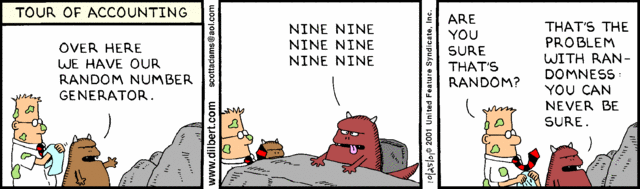
\includegraphics[width=\textwidth]{images/random}
}
\end{minipage}%
%
\hfill
%
\begin{minipage}{0.25\textwidth}%
\visible<2->{

\includegraphics[width=\textwidth]{images/query}
}
\end{minipage}
\vfill
\begin{minipage}{0.25\textwidth}
\visible<3->{

\includegraphics[width=\textwidth]{images/observe}
}
\end{minipage}%
%
\hfill
%
\begin{minipage}{0.7\textwidth}%
\visible<4->{
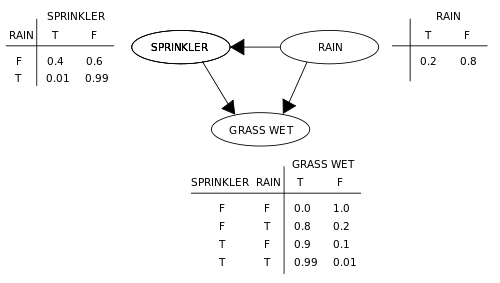
\includegraphics[width=\textwidth]{images/bayes}
}
\end{minipage}

\end{frame}


\note{

\begin{itemize}
\item Beispiel (Graph)
\item Modellierung in Church/ProbLog
\item Modellierung in Curry
\end{itemize}

}
\begin{frame}{Probabilistische Programmierung}{Bayes'sches Netz}

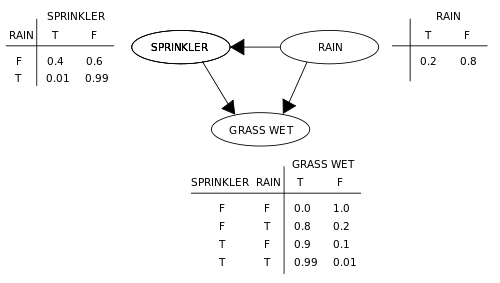
\includegraphics[width=\textwidth]{images/bayes}

\end{frame}


\begin{frame}[fragile]{Probabilistische Programmierung}{Einbettung in Curry}

\begin{semiverbatim}
data Dist a = Dist a Probability
data Probability = Prob Float
uniform :: [a] -> Dist a
scale :: [(a,Float)] -> Dist a
\end{semiverbatim}
  
\begin{semiverbatim}
playFixture :: Fixture -> Match
playFixture (Fixture team1 team2) =
  Match team1 team2 _

playFixtureP :: Fixture -> Dist Match
playFixtureP (Fixture team1 team2) =
  uniform [ match HomeVictory
          , match Draw
          , match AwayVictory]
 where match res = Match team1 team2 res
\end{semiverbatim}

\end{frame}


\begin{frame}{Probabilistische Programmierung}{Ausblick und Fazit}
\begin{minipage}{.48\textwidth}
\begin{itemize}
\item Suchstrategien (Tiefensuche, Breitensuche, Iterative Deepening)
\item Lazy Evaluation mit Sharing
\item call-time-choice
\item Nichtdeterminismus mittels Darstellung als Suchbaum
\item freie Variablen
\end{itemize}
\end{minipage}
%
\hfill
%
\begin{minipage}{.48\textwidth}
\begin{itemize}
\item Inferenzalgorithmen
\item explizites Speichern von Berechnung via $mem$
\item \emph{Many World}-Semantik
\item BDD zur Darstellung des Suchbaumes
\item Lazy Auswertung f\"ur Suchbaum
\item Delimitted Control als Optimierung
\end{itemize}
\end{minipage}

\end{frame}

\end{document}